\chapter{Detection of Adversarial Samples}
    \section{Misure di Difesa: Rilevamento di \textit{Adversarial Samples}}
        Per contrastare il fenomeno degli \textit{adversarial samples}, una strategia efficace consiste nell’introduzione di un \textbf{rilevatore di adversarial samples} a monte del sistema di classificazione. In particolare, in questo lavoro è stato adottato un \textit{Binary Input Detector} (BID), una rete neurale binaria il cui compito è discriminare tra input \textit{benigni} (ovvero non manipolati) e input \textit{adversarial}.
        L’approccio adottato si basa sull’assunzione che gli adversarial examples, pur essendo visivamente simili agli originali, presentino caratteristiche distribuzionali diverse nello spazio delle rappresentazioni apprese dal modello. Queste differenze possono essere apprese da un classificatore binario, opportunamente addestrato su un dataset contenente sia immagini originali sia immagini avversarie generate con i diversi attacchi eseguiti in precedenza.
        Il detector utilizzato è stato pre-addestrato su immagini preprocessate a bassa risoluzione ($32\times32$ pixel), con una architettura compatibile con \texttt{TensorFlowV2Classifier} della libreria \texttt{ART}. La scelta di un modello leggero e binario consente una facile integrazione nella pipeline del sistema di riconoscimento, con un buon compromesso tra accuratezza, velocità e capacità di generalizzazione.

    \section{Adversarial Detection come difesa proattiva}
        Il rilevamento di input avversari è una delle strategie difensive più studiate nel campo della sicurezza dei sistemi di machine learning. A differenza delle tecniche di robust training, che cercano di rendere il modello principale intrinsecamente più resistente agli attacchi, i meccanismi di \textit{detection} agiscono come un filtro a monte del classificatore, con l’obiettivo di intercettare e bloccare campioni sospetti prima che possano compromettere il processo decisionale.
        Questa impostazione si inserisce nel più ampio contesto delle \textbf{difese proattive}, in cui l’input viene valutato separatamente rispetto alla rete target. In particolare, i \textit{Binary Input Detectors} (BID) rappresentano un approccio semplice ma efficace: un classificatore binario viene addestrato su un dataset contenente sia immagini originali che malevole, con l’obiettivo di imparare a distinguere le due distribuzioni.
        L’assunzione di fondo è che, anche se le perturbazioni sono impercettibili a livello visivo, esse modificano in modo sistematico le rappresentazioni interne apprese dal modello, generando anomalie statistiche sfruttabili dal rilevatore. Tuttavia, questa strategia non è priva di limiti, infatti un BID è fortemente dipendente dal tipo di attacchi osservati durante l’addestramento e può risultare meno efficace contro tecniche mai viste o particolarmente sofisticate. Inoltre, come evidenziato in letteratura, alcuni detector possono essere facilmente ingannati da attacchi \textit{transfer-based} oppure \textit{adaptive}, in cui l’attaccante è a conoscenza della presenza del detector e ne ottimizza la perdita in fase di generazione dell’attacco.
        Un ulteriore elemento critico riguarda la \textit{generalizzazione}, poichè il rilevatore potrebbe imparare a riconoscere pattern specifici di un attacco piuttosto che le proprietà generali degli adversarial samples. Ciò può portare a overfitting e a una drastica riduzione dell’efficacia su dataset reali o su attacchi fuori distribuzione.
        Nel contesto di questo progetto, l’uso di un BID pre-addestrato su immagini preprocessate a bassa risoluzione consente di valutare in modo controllato la capacità del detector di distinguere tra classi avversarie e legittime. Nonostante le limitazioni insite in questo approccio, i risultati ottenuti mostrano che, almeno nel dominio considerato e con attacchi di intensità moderata, la strategia di detection risulta efficace e rappresenta una valida prima linea di difesa contro input manipolati.
        Nel seguito, vengono descritte le procedure di preprocessing, addestramento e validazione del rilevatore, accompagnate da un'analisi quantitativa delle performance ottenute.

    \section{Implementazione del Detector}
        L’intero processo di implementazione del detector di adversarial samples, si articola in tre fasi principali: preprocessing dei dati, addestramento del modello e valutazione su un insieme di validazione.
        
        \subsection{Preprocessing e Costruzione del Dataset}
            I dati utilizzati per l’addestramento e la validazione del detector sono stati ottenuti a partire dal test set originale, composto da immagini \textit{benigne} di volti provenienti dal dataset VGGFace2. Le immagini, inizialmente nel formato $160\times160\times3$, sono state ridimensionate a $32\times32\times3$ per renderle compatibili con l’input richiesto dal modello di rilevamento.
            In parallelo, sono stati riutilizzati i campioni \textit{adversarial} generati mediante l’utilizzo dei sei attacchi eseguiti in precedenza: FGSM, BIM, PGD error-generic e le rispettive versioni \textit{targeted}. Per evitare problemi di bias, sono stati esclusi gli attacchi DeepFool e Carlini-Wagner, i quali non coprono l’intero test set.
            Per ciascun attacco, le immagini avversarie sono state preprocessate con la stessa procedura delle immagini originali. \\
            Il dataset finale per l’addestramento del detector è stato costruito unendo:
                \begin{itemize}
                    \item Immagini \textbf{benigne} con etichetta 0,
                    \item Immagini \textbf{adversarial} con etichetta 1.
                \end{itemize}
    
            \noindent La divisione tra training e validation set è stata effettuata mediante \texttt{train\_test\_split}, mantenendo la proporzione 80\% / 20\% . Al termine, i dati sono stati \texttt{mescolati} per evitare correlazioni tra ordine e label e quindi   ottenere maggior randomicità.
    
        \subsection{Addestramento del Detector}
            Il rilevatore è stato implementato tramite il wrapper \texttt{BinaryInputDetector} fornito dalla libreria ART. Al suo interno è impiegato un classificatore binario costruito come oggetto \texttt{TensorFlowV2Classifier}, caricato da un modello pre-addestrato salvato nel file \texttt{BID\_eps=0.05.h5}.
            L’addestramento è stato effettuato sul dataset binario costruito in precedenza, utilizzando una funzione di perdita binaria cross-entropy e l’ottimizzatore Adam con tasso di apprendimento 0.001. Sono state effettuate 10 epoche di training con batch size pari a 64.
    
        \subsection{Valutazione sul Validation Set}
            Il rilevatore è stato testato su un validation set costituito da 3374 immagini, di cui 482 appartenenti alla classe \textit{benign} e 2892 alla classe \textit{adversarial}, ottenute dagli attacchi citati in precedenza. I risultati della classificazione binaria sono sintetizzati nella matrice di confusione riportata in Figura~\ref{fig:conf_matrix}.
            Dall’analisi dei dati emerge un comportamento particolarmente conservativo da parte del modello: tutti i campioni benigni sono stati classificati correttamente, senza generare alcun falso positivo. Questo risultato è di particolare interesse per l’affidabilità di un sistema reale, poiché evita che input legittimi vengano bloccati erroneamente dal sistema di difesa. Tuttavia, circa il 24\% dei campioni adversarial (684 su 2892) non è stato rilevato, venendo etichettato erroneamente come benigno. Questo porta a un richiamo (\textit{recall}) per la classe adversarial pari al 76.36\%, mentre la precisione rimane perfetta (1.00), poiché tutti i campioni rilevati come falsi lo erano realmente.
            Complessivamente, il sistema raggiunge un’accuratezza dell’79.73\%, con un F1-score di 0.87 per la classe adversarial e 0.58 per la classe benign. Quest’ultima differenza riflette uno sbilanciamento nella strategia decisionale del modello, che tende a favorire la sicurezza rispetto all’usabilità: rileva con estrema cautela gli attacchi, evitando qualsiasi classificazione errata di input benigni, ma accetta il compromesso di non intercettare la totalità dei campioni avversari.
            L’immagine in Figura~\ref{fig:conf_matrix} illustra bene questo comportamento. I valori lungo la diagonale confermano la capacità del modello di apprendere le caratteristiche principali dei dati, mentre la presenza significativa di falsi negativi (684) nella parte inferiore sinistra evidenzia il margine di miglioramento nella generalizzazione su esempi avversari più sofisticati o meno evidenti.
            Nel complesso, i risultati ottenuti indicano che il rilevatore è in grado di operare in modo affidabile in contesti in cui è cruciale minimizzare i falsi allarmi. Tuttavia, per aumentare ulteriormente la robustezza, potrebbe essere utile integrare strategie complementari, come tecniche di data augmentation.
    
        \begin{figure}[H]
            \centering
            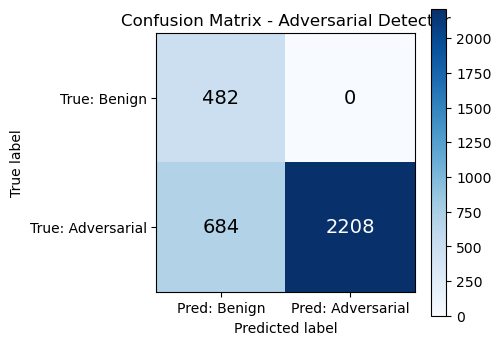
\includegraphics[width=0.6\textwidth]{images/confusionMatrix.png}
            \caption{Matrice di confusione del detector sul validation set.}
            \label{fig:conf_matrix}
        \end{figure}